Este capítulo aborda a execução do método proposto por este trabalho e a análise dos resultados obtidos pelos experimentos realizados a fim de verificar a viabilidade do projeto, bem como sua eficiência.

\section{Planejamento dos experimentos}\label{sec:result_planejamento}
O intuito desta avaliação experimental é verificar a capacidade do sistema \productname{} de classificar as ações do usuário a partir da leitura de sensores, e exibir um modelo virtual animado que demonstra esses dados. Para tal, foi necessário o desenvolvimento de um protótipo físico para a captura dos movimentos e de um \textit{software} para visualização.

\subsection{Captura dos movimentos}\label{sec:result_captura}
O protótipo para captura de dados consiste em um Arduino Nano, um sensor MPU-6050 e um sensor flexível, conectados conforme o esquema da \autoref{fig:result_schem}. 

\begin{figure}[ht]
	\caption{\label{fig:result_schem}Esquema das conexões dos sensores ao Arduino}
	\begin{center}
	    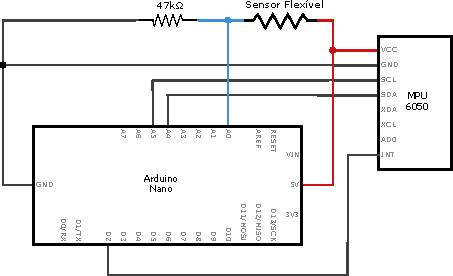
\includegraphics[width=.8\textwidth]{resources/result_schem}
	\end{center}
	\legend{Fonte: Elaborada pelo autor}
\end{figure}

Todos esses equipamentos foram fixados em uma joelheira de material flexível não rígido, como visto na \autoref{fig:result_prototipo}, com o MPU-6050 (b) posicionado acima do joelho, e o sensor flexível (a) posicionado atrás do joelho. Este sensor teve de ser posicionado desta forma devido ao seu comprimento de apenas 2,2 polegadas, pois seu posicionamento na parte frontal do joelho impediria que a resistência do sensor variasse o suficiente.

\begin{figure}[ht]
	\caption{\label{fig:result_prototipo}Protótipo com o sensor flexível (a) e o MPU-6050 (b) conectados ao Arduino Nano}
	\begin{center}
	    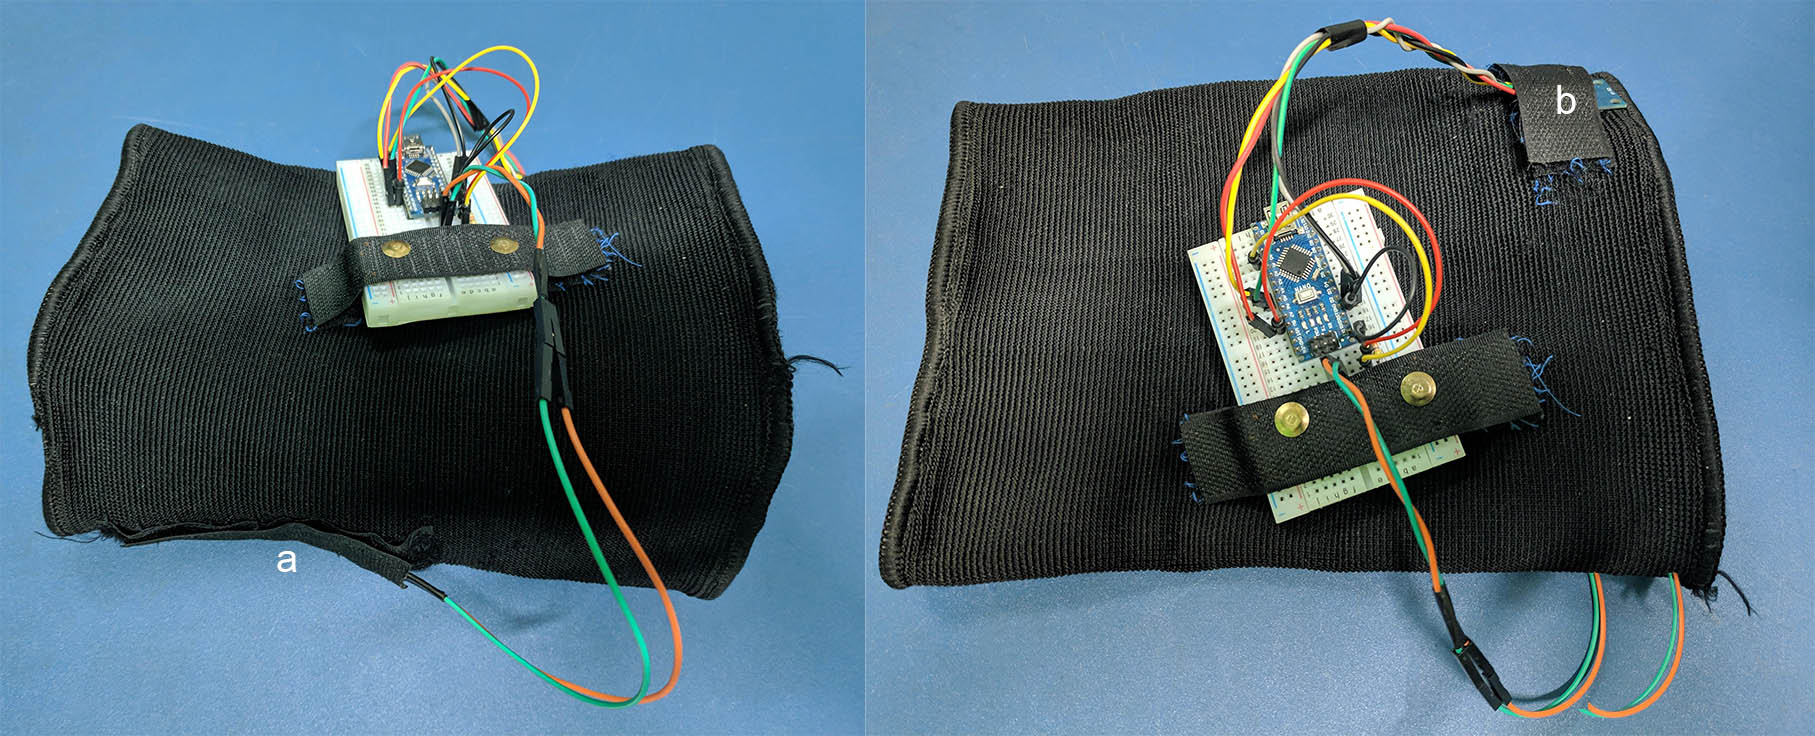
\includegraphics[width=.8\textwidth]{resources/result_prototipo}
	\end{center}
	\legend{Fonte: Elaborada pelo autor}
\end{figure}

Para que sejam possíveis a leitura e a classificação dos dados capturados, o Arduino é conectado via USB em um computador que executa o \textit{software} de simulação. Os dados do giroscópio, acelerômetro e resistência do sensor flexível, respectivamente, são enviados continuamente via comunicação serial pelo \textit{software} carregado no Arduino.

\subsection{\textit{Software} de simulação}\label{sec:result_simulacao}
O sistema de simulação é executado em um computador e foi desenvolvido na linguagem Python, para facilitar o uso da ferramenta scikit-learn. O programa é composto por diversos componentes que se integram para realizar diferentes atividades: leitura dos dados, através da biblioteca \textit{pyserial}\footnote{\url{https://github.com/pyserial/pyserial}}; gravação dos dados em arquivos; classificação dos dados, utilizando scikit-learn; e a exibição 3D com o uso das bibliotecas \textit{PyOpenGL}\footnote{\url{http://pyopengl.sourceforge.net/}} e \textit{pygame}\footnote{\url{https://www.pygame.org/}}.

A simulação animada em 3D, exibida na~\autoref{fig:result_simulacao} mostra em tempo real o movimento realizado pelos dois sensores e, após a captura dos dados, mostra também a ação realizada na prótese simulada, baseado na classificação dos dados de movimento.

\begin{figure}[ht]
	\caption{\label{fig:result_simulacao}Visualização da posição da perna do usuário e simulação da prótese}
	\begin{center}
	    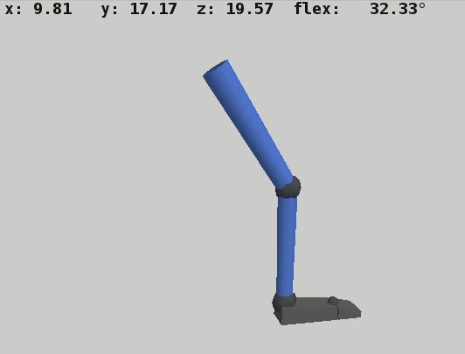
\includegraphics[width=.8\textwidth]{resources/result_simulacao}
	\end{center}
	\legend{Fonte: Elaborada pelo autor}
\end{figure}

\section{Execução dos experimentos}\label{sec:result_execucao}

Com o protótipo confeccionado e os \textit{softwares} desenvolvidos, deu-se início à captura de dados dos sensores, na qual observou-se que os melhores dados a serem usados para a classificação dentre os disponíveis seriam os valores do acelerômetro e do sensor flexível, ignorando a orientação do giroscópio, que ainda é utilizada para orientar a simulação.

Foram selecionados dois\todo{foi o que deu tempo}{ } indivíduos com os membros intactos para gerar o conjunto de dados que seria utilizado para a classificação. O dispositivo vestível foi utilizado na perna direita e foi solicitado para que cada um deles caminhasse em linha reta, enquanto era capturado o estado da transição de cada uma das ações.

A captura foi feita a partir de um cabo USB conectado a um \textit{notebook} (com um processador Intel i7-7500U, que conta com \textit{clock} de até \(3{,}5\) GHz e \(8\) GB de RAM) no sistema operacional Manjaro Linux\footnote{\url{http://manjaro.org/}}, estabelecendo comunicação serial com o programa.

As ações definidas para este experimento foram apenas voltadas à detecção de uma caminhada plana, classificando cada um dos passos de cada perna\todo{só não deu tempo}. Ou seja, além do estado de repouso (estado 0), foram armazenados o ponto em que a perna esquerda estava para frente (estado 1), e o ponto em que a perna direita estava para frente (estado 2), ilustrados pela \autoref{fig:result_estados}. Ao todo, foram realizadas \todo{De novo, foi o que deu tempo}140 amostras.

\begin{figure}[ht]
	\caption{\label{fig:result_estados}Demonstração das três ações capturadas para a classificação}
	\begin{center}
	   % 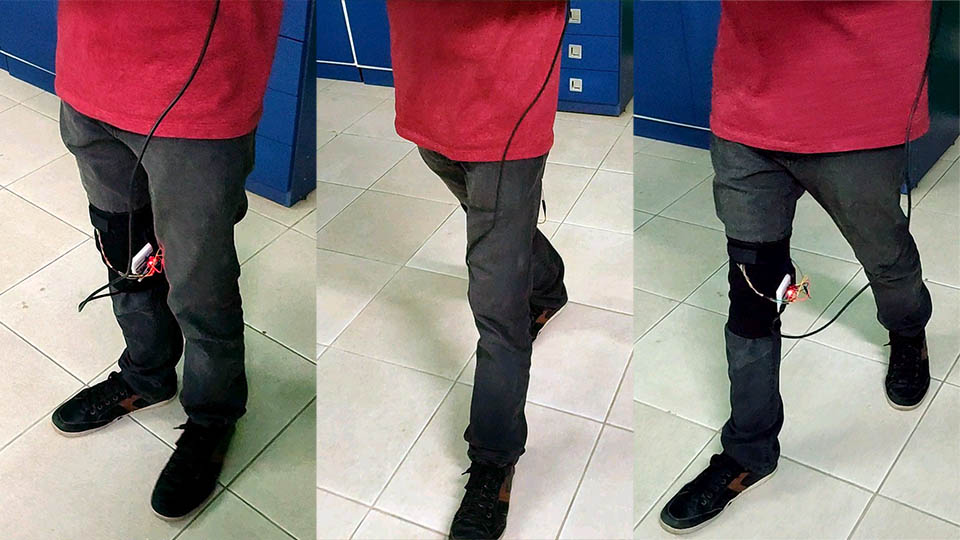
\includegraphics[width=\textwidth]{resources/result_estados}
	   \missingfigure[figwidth=\textwidth]{Tirar 3 fotos em cada uma das posições para ilustrar as ações no texto (ou só capturar do vídeo de exemplo)}
	\end{center}
	\legend{Fonte: Elaborada pelo autor}
\end{figure}

\subsection{Análise dos resultados}\label{sec:result_analise}

A partir dos dados coletados dos usuários, verificou-se através de validação cruzada que a árvore de decisões CART seria o algoritmo mais apropriado dentre os disponíveis no scikit-learn, com acurácia de aproximadamente \(94{,}7\%\) para os dados selecionados, como pode ser visto no gráfico da \autoref{fig:result_accuracy_plot}.

\begin{figure}[ht]
	\caption{\label{fig:result_accuracy_plot}Gráfico de acurácia do algoritmo CART}
	\todo[inline]{Tentar gerar um gráfico mais interessante: \url{https://scikit-learn.org/stable/auto_examples/model_selection/plot_cv_indices.html}}
	\begin{center}
	    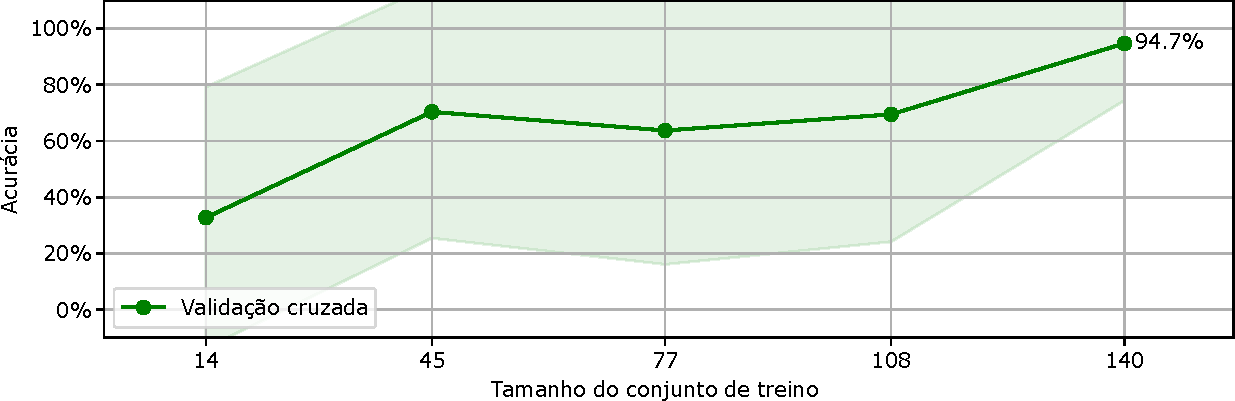
\includegraphics[width=\textwidth]{resources/result_accuracy_plot}
	\end{center}
	\legend{Fonte: Elaborada pelo autor}
\end{figure}

Ao longo dos experimentos realizados, notou-se que o sensor flexível ficou cada vez menos preciso, o que tornou a simulação um pouco menos realista, mas não impediu que os dados fossem classificados e as ações previstas.

Além disso, observou-se que com a coleta realizada não foi possível gerar um conjunto de dados genérico que funcionasse para todos os indivíduos. Portanto, cada usuário teria que gerar um conjunto de dados que seria utilizado para prever os próprios movimentos. Os conjuntos de dados compilados falham ao ser usados para predizer os movimentos de qualquer um dos sujeitos de teste. Suspeita-se que isso se deve à diferença no posicionamento dos sensores que acaba ocorrendo pelas diferenças físicas entre os indivíduos, o que poderia ser resolvido com uma joelheira.